\chapter{Grundlagen}

Das Grundlagenkapitel gibt eine Einführung und Übersicht über die verwendeten Begriffe und Konzepte, auf die im Weiteren der Arbeit zurückgegriffen wird. Zunächst wird die Darstellung von Bildern behandelt und anschließend die Erhebung von charakteristischen Merkmalen aus Bildern, den Features. Zur Detektion und Extraktion von Features aus Bildern haben sich zahlreiche verschiedene Verfahren etabliert. Von diesen wird der SIFT Feature Detektor und Deskriptor näher betrachtet, da er im Weiteren als Basis für die Feature Gewinnung dient. 
Es werden anschließend zwei Modelle vorgestellt, die eine Klassifikation von Bildern auf Basis von Features ermöglichen. Das Bag of Visual Words Modell wurde aus dem Bereich Information Retrival adaptiert. Es wird anhand der Features von Trainingsbildern eins visuelles Vokabular gelernt, dass zur Klassifizierung von Bildern dient. Alternativ zu diesem Ansatz wird der Autoencoder vorgestellt. Ein Autoencoder ist ein spezielles neuronales Netzwerk, dass selbständig eine komprimierte Darstellung der Eingabe, in diesem Fall der Features, lernt. 
Im letzten Teil wird auf die Berechnung allgemein mathematischer Probleme auf Grafikkarten, das GPGPU Programming eingegangen. Durch den Einsatz von Grafikkarten können Berechnungen gerade bei großen Datenmengen stark beschleunigt werden, da diese massiv parallel auf den Daten arbeiten. Mit Nvidias cuda wird eine Sprache eingeführt, mit der sich Modelle wie der Bag of Visual Words und Autoencoder auf Nvidia Grafikkarten ausführen lassen.

\section{Bilder und Features}

Zunächst wird definiert wie ein Bild mathematisch aufgefasst wird um eine effiziente Verarbeitung zu ermöglichen. Jedes Verfahren erwartet ein Bild als Eingabe. Verändern Algorithmen ein Bild, so geben sie die bearbeite Version wieder aus. Bei Analysen hingegen wird ein Bild nicht verändert, es wird auf Muster untersucht und die gefundenen Eigenschaften zurückgegeben. Diese Eigenschaften werden Features genannt. Der Prozess der Featuregewinnung ist in Detektion und Extraktion unterteilt und wird im Anschluss behandelt.

\subsection{Bilder}

Bei einem digitalen Bild handelt es sich um eine Matrix $I(x, y)$. Die Anzahl der Spalten $m$ und Zeilen $n$ entspricht dabei den Dimensionen des Bildes in Pixeln. Hier bezeichnen $(x, y)$ diskrete Koordinaten der Matrix und somit die einzelnen Pixel des Bildes. Die Darstellung in Matrixform eignet sich  sehr gut für Transformationen und Analysen des Bildes. Solche Verfahren betrachten oft jeden Pixel und seine Nachbarschaft. Die direkte Nachbarschaft eines Pixels ist eine $3 \times 3$ Matrix (mit dem Pixel als Zentrum), die alle unmittelbar anliegenden Pixel beinhaltet.

$$
I(x, y) = \begin{bmatrix}
i_{0, 0}   & i_{0, 1}	& \dots	 & i_{0, n-1}   \\
i_{1, 0}   & i_{1, 1}   & \dots  & i_{1, n-1}   \\
\vdots	   & \vdots 	& \ddots & \vdots       \\
i_{m-1, 0} & i_{m-1, 1} & \dots	 & i_{m-1, n-1}
\end{bmatrix}
$$ 

Abhängig vom Typ des Bildes, besitzen die Pixel eine andere Struktur. In der Bilderverarbeitung und im Weiteren dieser Arbeit werden meist folgenden Arten von Bildern verwendet:
\begin{itemize}
	\item \textbf{Monochromatische Bilder} Diese Bilder werden nur in Graustufe dargestellt, daher besitzt ein Pixel genau einen Intensitätswert.
	\item \textbf{Multispektrale Bilder} Jeder Pixel besitzt einen Vektor an Werten. Im Falle eines Farbbildes enthält der Vektor drei Intensitätswerte für rot, grün und blau.
\end{itemize}
Die Intensität eines Pixels bzw. die Intensität seiner Vektoren wird mit acht Bit dargestellt und umfasst daher 256 mögliche Werte. Diese Werte werden im Folgenden normalisiert im Intervall $[0, 1]$ angegeben.

\begin{itemize}
	\item TODO: Grafik mit beliebigem Bild und Abbildung von Pixel in Raster mit Koordinaten (x, y) ? 
\end{itemize}

\subsection{Feature Detektion und Extraktion}

Um Bilder zu vergleichen werden charakteristische Merkmale dieser betrachtet, die sogenannten Features. Ein Feature ist ein allgemeiner Begriff und enthält je nach Verfahren unterschiedliche Informationen. Dies ist notwendig, da nicht nur die Position oder Intensität eines Pixels, sondern auch generelle Eigenschaften von Interesse sind. Globale Verfahren berücksichtigen bei der Bewertung jeden Pixel des Bildes gleichermaßen, lokale hingegen betrachten nur ein kleine Fenster des Bildes, also einen Pixel und seine Nachbarschaft. Die Suche nach globalen Merkmalen, die ein Bild charakterisieren, kann aber keine Objekte und Details im Bild berücksichtigen. Hierfür eignet sich die Extraktion von lokalen Features. Um Objekte aus unterschiedlichen Perspektiven und in verschiedenen Größen wieder zu erkennen, ist es notwendig, dass die Features affin invariant sind. Folgende Abbildung zeigt dasselbe Objekt, jedoch rotiert, skaliert und verschoben. Ein Algorithmus sollte mit hoher Wahrscheinlichkeit erkennen, dass es sich hier um dasselbe Objekt handelt.

BEISPIEL BILD

Die Gewinnung der Features ist in zwei Schritte aufgeteilt: 
\begin{itemize}
	\item \textbf{Detektion} Zuerst ermittelt ein Detektor Muster im Bild. Die untersuchten Muster sind abhängig vom Detektor Pixel, Linien oder Regionen einer Nachbarschaft. Hierfür wird jeder Pixel und seine Nachbarschaft betrachtet und entschieden ob es sich um einen \textit{key point} handelt. Ein Detektor gibt als Ergebnis alle Pixel zurück, bei denen es sich um {key points} handelt. Manche Verfahren geben zusätzlich zu den \textit{key points} auch Eigenschaften wie die Orientierung oder den Maßstab aus. Um praktisch einsetzbar zu sein, muss ein Detektor ein Feature, dass in verschiedenen Bildern auftaucht, zuverlässig erkennen. Hier sollte aber die angestrebte Allgemeinheit berücksichtigt werden: Ein Feature Detektor für medizinische Bilder kann spezieller Annahmen treffen, als einer für eine allgemeine Bildsuche.
	\item \textbf{Extraktion} Die Feature Extraktion erzeugt aus den vom Detektor gefundenen \textit{key points} den Deskriptor. Ein Feature Deskriptor ist eine kompakte Darstellung eines Features. Die \textit{key points} und deren Eigenschaften werden in Zahlen kodiert. Oft wird hier nicht nur ein Feature erzeugt, sondern ein Feature-Vektor, der auch Deskriptoren der Nachbarschaft des \textit{key points} enthält. Von einem Deskriptor ist es wünschenswert, dass er affin invariant ist. Somit kann das Feature auch erkannt werden, wenn das Bild rotiert, verschoben oder skaliert wurde.
\end{itemize}

Im Folgenden werden zwei Verfahren zur Feature Detektion und Extraktion vorgestellt, die sich in der Praxis bewährt haben und teilweise affine Invarianz aufweisen. Das Histogram of Oriented Gradients ist weit verbreiteter ein Feature Deskriptor, der sich im Breich der Objektdetektierung bewährt hat. SIFT ist ein von Lowe entwickeltes Verfahren zur Feature Extraktion und Detektion. Bei der Detektion von Features werden Rotationen, Skalierungen und Translationen von gefundenen Features erkannt und diese durch Den Deskriptor als ein Histogramm der Orientierungen dargestellt.\cite{ifd2016}

\begin{figure}
	\centering
	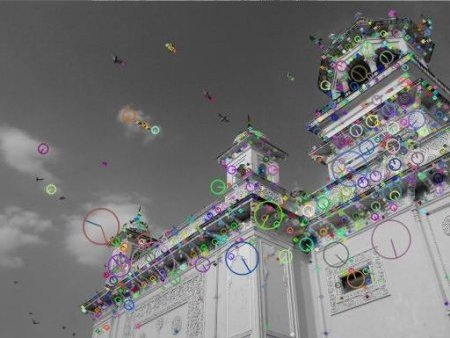
\includegraphics[scale=0.7]{images/sift_keypoints.jpg}
	\caption{Gefundene \textit{key points} in einem Bild farblich hervorgehoben (SIFT Detektor)}
	\label{img:interset_points}
\end{figure}

\subsection{Histogram of Oriented Gradients}

Um den Begriff zu klären, werden zunächst das Histogramm und Gradienten von Bildern (\textit{image gradients}) eingeführt. Ein Histogramm ist eine diskrete Funktion, welche die Häufigkeitsverteilung einer Menge abbildet. Hierfür wird jeder Wert der Menge einer Klasse zugeordnet. Jede Klasse umfasst einen vorher definierten Wertbereich. Als einfachen Fall dient hier die Verteilung der Pixel eines Bildes auf die Intensitäten. Bei einem monochromatischen Bild liegen 256 Klassen vor. Beim bilden des Histogramms wird jeder Punkt betrachtet und der Zähler der Klasse um eins inkrementiert, in deren Wertebereich der Intensitätswert des Punktes fällt. Ein Histogramm ist normalisiert, wenn die Anzahl der Werte einer Klasse durch die Anzahl der Gesamtwerte dividiert wird.
In Abbildung \ref{img:hist} sind im Wesentlichen zwei Bereiche zu erkennen: ein sehr hellerer Hintergrund und eine dunkle Katze, die den Großteil des Bildes ausmacht. Dies spiegelt sich auch im Histogramm wieder: Es ist eine große Mengen an Punkten im dunklen Bereich vorhanden (Intensität < 128) und eine kleine, extreme Häufung im hellen Bereich.

\begin{figure}
	\centering
	\includegraphics[scale=0.8]{images/big_cat.png}
	\caption{Graustufenbild und Verteilung der Intensitätswerte}
	\label{img:hist}
\end{figure}

Ein Gradient gibt die Intensitätsänderung eines Pixels und seiner Nachbarschaft in einer Richtung an. Die dominante Richtung entspricht einer großen Intensität. 

\begin{itemize}
	\item TODO: Histogram of Oriented Gradients
 	\item TODO: Abbildung
\end{itemize}

\subsection{Scale-invariant feature transform}

SIFT ist ein Feature Detektor und Deskriptor der 1999 von Lowe entwickelt wurde. Die von SIFT entdeckten Features sind (affin?) invariant und beschreiben die Nachbarschaft eines \textit{keypoints}. Der Algorithmus ist in vier Schritte unterteilt:

\begin{enumerate}
	\item \textbf{Detektion von Extremen im Maßstab} Die \textit{keypoints} werden durch einen Difference of Gaussians (DOG) Filter ermittelt. Das Bild wird durch eine Konvolution mit einem gausschen Kernel $G(x, y, d)$ geglättet, wobei $d$ die Standardabweichung ist. Dadurch das nur räumliche Informationen höherer Bereiche unterdrückt werden, fungiert dies als Band Pass Filter und hebt so die Sichtbarkeit von Kanten hervor. Der Lapalacien of Gaussian wird dann durch die Differenz zweier Gaussians berechnet. Dabei ist die Standardabweichung des Minuenden $k$ mal größer, als die des Subtrahenden. In der Praxis hat sich beim Einsatz in SIFT der Wert $k = 1.4$ bewährt. Die Extrempunkte aus einer Reihe von DOG Abbildungen sind dann die Punkte, die ein lokales Minimum oder Maximum besitzen. 
\begin{figure}
	\centering
	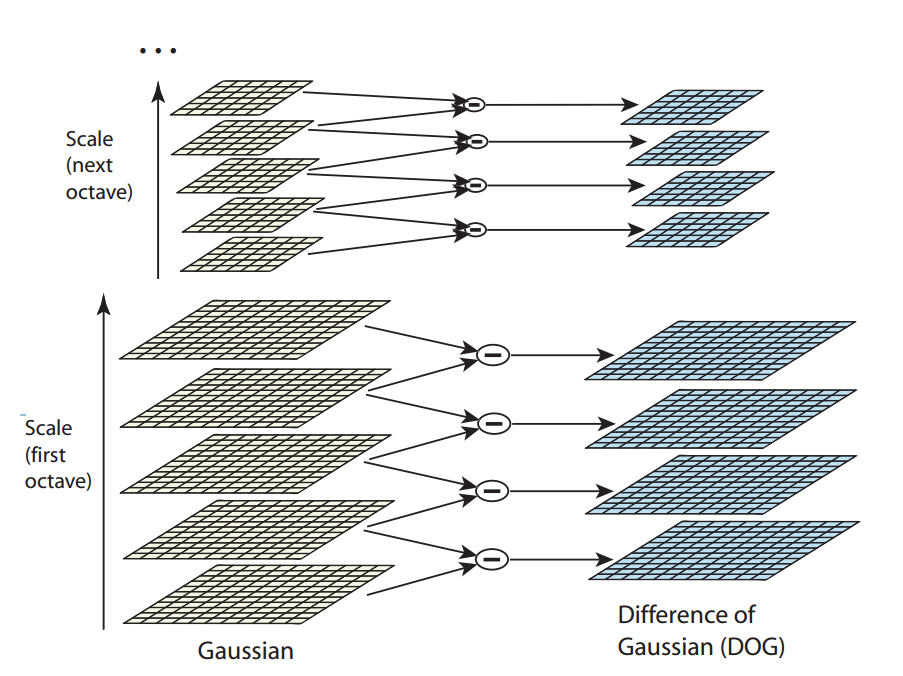
\includegraphics[scale=0.5]{images/sift_dog.png}
	\caption{Difference of Gaussians Operator, Abbildung aus \cite{dif2004}}
	\label{img:sift_dog}
\end{figure}	
	
	\item \textbf{Keypoint Lokalisierung} Nicht alle Kandidaten werden zu \textit{keypoints}. Jeder Kandidaten muss einer Reihe von Stabilitätsmaßen genügen. Befindet sich ein Punkt auf einer Kante oder besitzt einen zu geringen Kontrast, wird er aussortiert. Dies wird durch eine Taylor Expansion zweiter Ordnung mit Ursprung im \textit{keypoint} durchgeführt.
	\item \textbf{Bestimmung der Orientierung} Bei dem Aufbau des Feature Vektoren pro \textit{key points} wird die lokale Orientierung abgeschätzt. Auf diese Weise sind die SIFT Deskriptoren invariant gegenüber Rotationen. Der SIFT Algorithmus berechnet ein Histogramm der Orientierung der Gradienten. Hierfür werden zufällig Punkte aus der Nachbarschaft ausgewählt. Der Extremwert des Histogramms wird hier als dominante Orientierung verwendet.
	\item \textbf{Deskriptor} Für jeden durch den Detektor gefundenen \textit{keypoint} wird nun ein Featurevektor gebildet. Der Featurevektor enthält Informationen über die Nachbarschaft in Form der Gradienten eines jeden Punktes in der Nachbarschaft. Das Fenster für die Auswahl der Nachbarschaft wird auf dem \textit{keypoint} zentriert und in vier Teilfenster unterteilt. Die Gradienten in allen Teilfenster werden in acht Richtungen quantisiert, sodass der resultierende Deskriptor 128 Dimensionen enthält.
\begin{figure}
	\centering
	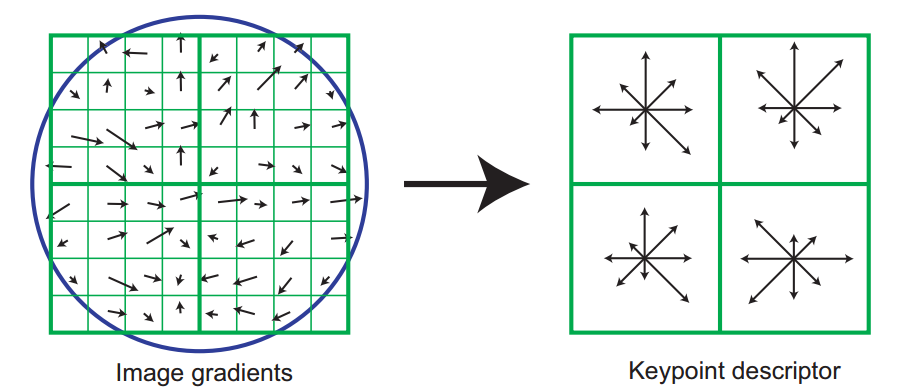
\includegraphics[scale=0.4]{images/sift_desc.png}
	\caption{Ein $8 \times 8$ Sample aus dem ein $2 \times 2$ Deskriptor berechnet wird, Abbildung aus \cite{dif2004}}
	\label{img:sift_desc}
\end{figure}	
	
\end{enumerate}

SIFT ist äußerst robust, da Änderungen im Grenzwert von Position und Orientierung den Feature Vektor kaum beeinflussen. Der Deskriptor besitzt zwar keine affine Invarianz, in praktischen Anwendungen werden jedoch auch mit skalierten, rotierten und verschobenen Objekten gute Ergebnisse erzielt. Auch im Vergleich zu anderen Algorithmen (SUSAN, SURF, ...) schneidet SIFT gut ab, meist mit besseren Ergebnissen. Die Konstruktion des Deskriptors ist allerdings sehr aufwendig und er weist eine hohe Dimensionalität auf. 

\begin{itemize}
	\item TODO: SIFT-PCA / Clustering erwähnen
	\item TODO: DOG näher erläutern, mathematische Notation?
\end{itemize}

\section{Bag of Visual Words}

Das Bag of Words Modell stammt aus dem Bereich Information Retrival und wird zur Klassifizierung von Dokumenten genutzt. Es wird das Auftreten jedes Wortes in eine Dokument gezählt und durch die Anzahl aller Wörter im Vokabular dividiert, um so einen normalisierten Wert zu erhalten, welcher die relative Häufigkeit eines Wortes angibt. Das Vokabular wird \textit{Codebook} genannt, die Wörter sind die \textit{Codewords}.
Dieses Modell wurde von der Computer Vision adaptiert um Bilder zu klassifizieren. Die Features können aber nicht direkt statt der Worthäufigkeit verwendent werden: Ein Wort ist ein diskreter Wert der direkt verglichen werden kann, ein Feature hingegen ist ein hochdimensionaler Vektor, der Eigenschaften beschreibt. Um konkrete Werte zu erhalten, ist es notwendig die Vektoren zu quantisieren. Die quantisierten Vektoren entsprechen dann den \textit{Codewords} und werden in diesem Kontext auch \textit{Visual Words} genannt. Um \textit{Visual Words} aus einer Menge von Trainingsbildern zu erhalten, werden die Feature-Vektoren durch ein Clustering Verfahren gruppiert. Die Idee ist, dass ähnliche Vektoren nah beieinander im Raum liegen und somit in die gleich semantische Kategorie gehören. Durch einen Clustering Algorithmus wie k-means kann die Größe des \textit{Codebooks} bestimmt werden. Die Größe des \textit{Codebooks} ist ein wichtiger Parameter. Wird für $k$ ein große Zahl gewählt, wird ein Vokabular von Exemplaren aufgebaut, ein kleines $k$ hingegen erkennt eher Kategorien.
Wurde das \textit{Codebook} erzeugt, können anschließend Bilder klassifiziert werden. Hierfür werden wieder die Features eines Bildes extrahiert und nun für jedes der Cluster bestimmt, der diesem am nächsten ist. Das Ergebnis ist eine Verteilung der relativen Häufigkeit der \textit{Visual Words} des Bildes. TODO: Klassifizierung

\subsection{k-means Clustering}

Unter k-means Clustering werden Algorithmen zusammengefasst, die eine Menge Vektoren durch Zuweisung in $k$ vorgegeben Gruppen einteilen, die sogenannten Cluster. Aus den Vektoren werden initial $k$ Stück ausgewählt, die als anfängliche Zentren der Cluster dienen. Ein k-means Algorithmus ordnet nun iterativ jeden Vektor dem Cluster zu, dessen Varianz sich bei Aufnahme des Vektors am wenigsten erhöht. Aus diesem Grund setzt das k-means Clustering einen euklidischen Raum voraus.
Soll ein globales Optimum gefunden werden, so ist k-means NP-schwer. Praktische Implementierungen approximieren daher meist die Zentren der Cluster wie der Algorithmus von Llyod. Zunächst beginnt Llyod's Algorithmus mit einer Initialisierung. Schritt zwei und drei werden dann solange wiederholt, bis der Algorithmus konvergiert, also die Vektor-Cluster-Zuordnung sich nicht mehr ändert, oder eine maximale Anzahl an Iterationen erreicht wurde: 

\begin{enumerate}
	\item \textbf{Initialisierung} Es werden zunächst $k$ zufällige Vektoren als Cluster ausgewählt
	\item \textbf{Zuordnung}: Von den verbleibende Vektor wird nun mit jedem Cluster die neue Summe der Varianzen bei Aufnahme des Vektors berechnet. Es wird der Vektor dem Cluster zugeordnet, dessen Varianz sich am geringsten bei Aufnahme des Vektors erhöht.
	\item \textbf{Vektoren zuweisen}: Die Zentren den Cluster werden neu berechnet, um den neu zugeordneten Vektor in Folgeberechnungen miteinzubeziehen.
\end{enumerate}

Im Folgenden Beispiel werden zur Veranschaulichung zweidimensionale Vektoren, Punkte im Raum, betrachtet. Dieser Prozess läuft für höhere Dimensionen unter Berücksichtigung der Distanzmetriken analog ab, wenn sich die Vektoren im euklidischen Raum befinden. Als $k$ wird hier drei gewählt. Der Erste Cluster muss zufällig gewählt werden, da keine Informationen vorliegen, auf Basis derer eine gute Entscheidung getroffen werden kann. Als erstes wird der Punkt 4 gewählt. Im nächsten Schritt bestimmen wir den Punkt der am weitesten von Punkt 4 entfernt ist. Berechnet man die Distanz für alle Punkte, so sind Punkt 5 und 10 beide am weitesten und gleich weit von Punkt 4 entfernt. In diesem Fall wird zufällig Punkt 10 gewählt. Da nach ein Cluster gefunden werden muss wird nun die Distanz von jedem verbleibendem Punkt zu Punkt 4 und 10 bestimmt. Dieser Schritt liefert Punkt 1 als initialen Mittelpunkt für den dritten Cluster. \cite{mmd2011}

\begin{itemize}
	\item TODO: Abbildung mit Clustern, kürzere Erklärung fürs Beispiel
	\item Confusion Matrix um Matching zu bestimmen? 
\end{itemize}

\section{Autoencoder}

Ein Autoencoder ist ein spezielles neuronales Netzwerk. Diese Netze werden für das unbeaufsichtigte Lernen einer komprimierten Darstellung von Daten genutzt. Zunächst wird hierfür ein Überblick über das Themengebiet der neuronale Netze im Allgemeinen gegeben und anschließend die Funktionsweise eines Autoencoders erläutert. Darauf aufbauend werden zwei Erweiterungen des Autoencoders vorgestellt, um Rauschen in den Daten und besonders tiefe Netzwerke berücksichtigen.

\subsection{Neuronale Netze}

Neuronale Netze (ANN, KNN, NN) sind dem Aufbau und der Funktionsweise der Neuronen des menschlichen Gehirns nachempfunden. Es wird eine Menge von künstlichen Neuronen genutzt um eine Lösung für ein Problem zu gestalten. Erste theoretische Überlegungen tauchten bereits in den 40er Jahren auf. Durch die wachsende Rechenleistung und neue Forschungsgebiete wie Deep Learning und Machine Learning finden neuronale Netze seit Mitte der 80er Jahre vermehrt praktische Anwendung und akademische Zuwendung. Dadurch das neuronale Netze von Natur aus hoch parallel arbeiten, eignen sie sich vor allem für parallele Architekturen und die Verarbeitung großer Datenmengen. 
Ein neuronales Netz besteht aus einer Menge Neuronen die in Schichten im Netzwerk angeordnet sind. Jedes Neuron besitzt einen Aktivierungszustand und einen Schwellwert, von denen abhängt, ob ein Signal weitergeleitet wird. Neuronen benachbarter Schichten sind vollständig durch gewichtete Kanten miteinander verbunden. Diese Beziehung wird in einer Gewichtsmatrix ausgedrückt. Neuronen zwischen denen dann keine Verbindung vorhanden ist, besitzen das Gewicht 0. 
Das Netz verarbeitet ein Signal, welches hier als Vektor $x \in [0,1]^n$ mit Dimension $n$ dargestellt wird. Die erste Schicht des Netzwerks, der \textit{Input layer}, leitet das Signal nur an die nächste Schicht weiter und besitzt daher $n$ Neuronen. Die letzte Schicht, der \textit{Ouput layer}, dient zur Ausgabe des Ergebnisvektors $z \in [0,1]^m$, wobei $m$ die Größe des Vektors angibt. Zwischen diesen beiden Schichten können sich beliebig viele \textit{Hidden layer} befinden. Die \textit{Hidden layer} bilden somit den Kern des Netzes, deren Kantengewichtungen, Kanten und Neuronen selbst durch während eines Lernprozess angepasst werden.

\begin{figure}
	\centering

	\begin{tikzpicture}[shorten >=1pt,->,draw=black!50, node distance=\layersep]
    \tikzstyle{every pin edge}=[<-,shorten <=1pt]
    \tikzstyle{neuron}=[circle,fill=black!25,minimum size=17pt,inner sep=0pt]
    \tikzstyle{input neuron}=[neuron, fill=green!50];
    \tikzstyle{output neuron}=[neuron, fill=red!50];
    \tikzstyle{hidden neuron}=[neuron, fill=blue!50];
    \tikzstyle{annot} = [text width=6em, text centered]

    % Draw the input layer nodes
    \foreach \name / \y in {1,...,4}
        \node[input neuron, pin=left:$x_{\y}$] (I-\name) at (0,-\y) {};

    % Draw the hidden layer nodes
    \foreach \name / \y in {1,...,5}
        \path[yshift=0.5cm]
            node[hidden neuron] (H-\name) at (\layersep,-\y cm) {};

    % Draw the output layer node
    \node[output neuron,pin={[pin edge={->}]right:$z$}, right of=H-3] (O) {};

    % Connect every node in the input layer with every node in the
    % hidden layer.
    \foreach \source in {1,...,4}
        \foreach \dest in {1,...,5}
            \path (I-\source) edge (H-\dest);

    % Connect every node in the hidden layer with the output layer
    \foreach \source in {1,...,5}
        \path (H-\source) edge (O);

    % Annotate the layers
    \node[annot,above of=H-1, node distance=1cm] (hl) {Hidden layer};
    \node[annot,left of=hl] {Input layer};
    \node[annot,right of=hl] {Output layer};
	\end{tikzpicture}

	\caption{Beispiel eines neuronalen Netzes, dass vier Werte $x_{1,...,4}$ als Eingabe entgegennimmt. Der \textit{Input layer} leitet die Werte an jedes der fünf Neuron im \textit{Hidden Layer} weiter, was durch die Pfeile symbolisiert wird. Schließlich werden die Ausgaben des \textit{Hidden layers} an das einzige Neuron des \textit{Output layers} geschickt und von diesem das Ergebnis $z$ ausgegeben.}
	\label{img:n}
\end{figure}

Die Verarbeitung eines Signals in einem Neuron ist in Abbildung \ref{img:neuron} schematisch dargestellt und lässt sich in drei Schritte untergliedern:
\begin{itemize}
	\item \textbf{Propagierungsfunktion} Aus der Eingabe aller verbundenen Neuronen wird die Netzeingabe berechnet. Meist wird hier die gewichtete Summe zwischen Eingabe und Gewicht verwendet: $\sum_{i=1}^{} w_{i}x_{i} + b$.
	\item \textbf{Aktivierungsfunktion} Es wird der neue Aktivierungszustand des Neurons aus dem alten Zustand und der Netzeingabe berechnet. Häufig wird hier die logistische Funktion $s(x) = \frac{1}{1+e^-x}$ verwendet.
	\item \textbf{Ausgabefunktion} Wird ein Neuron aktiviert, so wird das resultierende Signal durch die Ausgabefunktion berechnet und an alle Neuronen in der folgenden Schicht weitergeleitet. Oft wird hier die Identitätsfunktion verwendet.
\end{itemize}

\begin{figure}
	\centering
	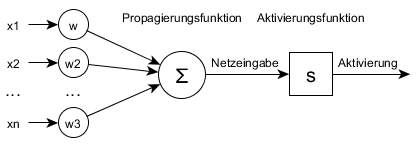
\includegraphics[scale=1.0]{images/neuron.png}
	\caption{Verarbeitung eines Signales in einem Neuron (ohne Ausgabefunktion) (Grafik überarbeiten)}
	\label{img:neuron}
\end{figure}

Wurde ein neuronales Netz konstruiert, folgt darauf die Trainingsphase. Durch das Training ist es möglich, dass ein Netzwerk Neuronen oder Verbindungen hinzufügt bzw. entfernt, den Schwellwert für die Aktivierung von Neuronen verändert oder die Gewichte zwischen Neuronen anpasst. Die Fehlerquote $F$ wird als die Summe der quadrierten Differenz zwischen dem angestrebten Ergebnis $r_{i}$ und der Ausgabe des Netzes $z_{i}$ berechnet:
$$ F()=\sum_{i=1}^{n} (r_{i} - z_{i})^2 $$
Um diese Veränderungen im Netz bekannt zu machen, wird das \textit{Backpropagation} Verfahren genutzt. \textit{Backpropagation} minimiert den Gradientenabstieg auf der Fehleroberfläche die $F$ aufspannt. Der Algorithmus geht in drei Schritten vor:

\begin{enumerate}
	\item \textbf{Forward Pass} Die Gewichte des Netzwerks werden initialisiert und eine Eingabe durch das Netz propagiert. Als Resultat liegt die Ausgabe $z_{i}$ für $i=1,...,n$ vor.
	\item \textbf{Berechnung} Die Summe der quadrierten Fehler $F$ wird berechnet.
	\item \textbf{Backward Pass} In diesem Schritt wird die Fehlerquote rückwärts durch das Netz propagiert. Die Gewichte an den Verbindungen zwischen Neuronen werden in Abhängigkeit ihres Einflusses auf den Fehler aktualisiert.
\end{enumerate}

\begin{itemize}
	\item TODO: Gradienten erläutern
	\item Die Formel für die Fehlerquote wahrscheinlich einfach entfernen oder sollte es hier stattdessen tiefer behandelt werden (Abbildung einer Fläche erzeugt durch F)?
\end{itemize}

\subsection{Funktionsweise}
Ein Autoencoder (AE) ist ein spezielles neuronales Netzwerk, dass eine komprimierte Kodierung der Eingabe lernt. Ein Autoencoder versucht die Daten zu rekonstruieren und kann daher unbeaufsichtigt lernen: Die rekonstruierten Daten können anhand einer Distanzmetrik mit den Originaldaten verglichen werden. Anschließend kann die Größe des Fehlers berechnet werden und durch \textit{Backpropagation} die Gewichtesmatrix aktualisiert werden.
Um die Originaldaten als Ergebnis erhalten zu können, muss die Anzahl der Neuronen des \textit{Input layers} der Anzahl der Neuronen im \textit{Output layer} entsprechen. Die Anzahl der Neuronen im \textit{Hiddenlayer} ist geringer, um die komprimierte Darstellung des Features zu erreichen. Werden mehrere \textit{Hiddenlayer} verwendet, so nimmt die Neuronenanzahl von Layer zu Layer ab um die Anzahl der Dimensionen weiter zu verringern. Dieser Vorgang ist die Enkodierung und liefert die gewünschte komprimierte Abbildung. Die Dekodierung ist umgekehrt aufgebaut, um das Original aus der komprimierten Repräsentation Schicht für Schicht zu rekonstruieren. Wie gut die Dekodierung gelungen ist, lässt sich dann anhand eines Vergleichs der Distanz des Original und der Rekonstruktion bewerten. Formal wird ein Eingabevektor $x \in [0,1]^n$ auf einen Vektor $y \in [0,1]^p$ durch $y = encode_{W,b}(x) = s(Wx + b)$ abgebildet. $W$ ist die Gewichtsmatrix $n \times p$ und $b$ der Bias-Vektor. Diese Parameter werden durch den Autoencoder optimiert. Die Rekonstruktion erfolgt durch die Dekodierungsfunktion: $z \in [0, 1]^n$ wird dann durch $z = decode_{W', b'}(y) = s(W'y + b')$ \cite{ssn1997}.

\begin{enumerate}
	\item TODO: Vorteile eines Autoencoders gegenüber anderen Verfahren (supervised, pretraining)
	\item TODO: Beispiel einbeziehen (\ref{img:example_ae})
	\item Weniger Mathematik oder anhand von Grafik mehr einbeziehen?
\end{enumerate}

\begin{figure}
	\centering

	\begin{tikzpicture}[shorten >=1pt,->,draw=black!50, node distance=\layersep]
    \tikzstyle{every pin edge}=[<-,shorten <=1pt]
    \tikzstyle{neuron}=[circle,fill=black!25,minimum size=17pt,inner sep=0pt]
    \tikzstyle{input neuron}=[neuron, fill=green!50];
    \tikzstyle{output neuron}=[neuron, fill=red!50];
    \tikzstyle{hidden neuron}=[neuron, fill=blue!50];
    \tikzstyle{annot} = [text width=6em, text centered]

    % Draw the input layer nodes
    \foreach \name / \y in {1,...,5}
        \node[input neuron, pin=left:$x_{\y}$] (I-\name) at (0,-\y) {};

    % Draw the hidden layer nodes
    \foreach \name / \y in {1,2,3}
        \path[yshift=-1.0cm]
            node[hidden neuron] (H-\name) at (\layersep,-\y cm) {};
    
    % Draw the output layer nodes
    \foreach \name / \y in {1,...,5}
        \node[output neuron,pin={[pin edge={->}]right:$z_{\y}$}, right of=H-3] (O-\name) at (\layersep,-\y) {};

    % Connect every node in the input layer with every node in the
    % hidden layer.
    \foreach \source in {1,...,5}
        \foreach \dest in {1,2,3}
            \path (I-\source) edge (H-\dest);

    % Connect every node in the hidden layer with the output layer
    \foreach \source in {1,2,3}
        \foreach \dest in {1,...,5}
        	\path (H-\source) edge (O-\dest);

    % Annotate the layers
    \node[annot,above of=H-1, node distance=2.0cm] (hl) {Hidden layer};
    \node[annot,left of=hl] {Input layer};
    \node[annot,right of=hl] {Output layer};
	\end{tikzpicture}

	\caption{Beispiel eines simplen Autoencoders}
	\label{img:example_ae}
\end{figure}

\subsection{Stacked Denoising Autoencoder}

Von Hinton and Salakhutdinov wurde 2006 das Konzept des Stacked Autoencoders eingeführt, um einige Probleme mit herkömmlichen Autoencoder zu überwinden. Bei Netzwerken mit mehr als einem Hidden Layer erzielt die Gradient Descent Methode bei der Rückpropagierung keine guten Ergebnisse mehr, aufgrund der Verzerrung er Gradienten. In vielen Ansätzen wurde auch eine zufällige Initialisierung der Gewichte gewählt. Hier besteht die Gefahr, dass der Algorithmus in einem lokalen Optimum verbleibt. Wenn die anfänglichen Gewichte hingegen bereits nah an einer guten Lösung liegen, sinkt die Wahrscheinlichkeit eines lokalen Optimums. Aus diesem Grund wurde das Pretraining für Autoencoder mit mehr als einer Schicht vorgeschlagen. Das Pretraining besteht aus zwei Schritten, von denen Schritt zwei und drei wiederholt werden, bis alle Gewichte trainiert sind.

\begin{enumerate}
	\item Es wird der unterste Autoencoder zuerst trainiert. Also der Autoencoder der aus dem \textit{Input-} und folgendem \textit{Hidden layer} besteht.
	\item Nun wird der Decoder des trainierten Autoencoders entfernt und ein neuen Autoencoder erzeugt. Dieser besitzt den \textit{Hidden layer} des trainierten Autoencoders als \textit{Input layer}.
	\item Das Training wird mit dem neuen Autoencoder fortgeführt.
\end{enumerate}

\cite{sda2010}

\begin{itemize}
	\item TODO: Abbildungen
	\item TODO: Denoising Autoencoder
\end{itemize}

\section{GPGPU Programmierung}

Der Begriff General Programming on Graphics Processing Units (GPGPU) beschreibt das Verwenden von Grafikkarten für Berechnungen, die nicht mit der Verarbeitung von grafischen Daten in Zusammenhang stehen. Zur Ausführung wird das Single Program Multiple Data (SPMD) Modell verwendet. Dies bedeutet, dass alle Prozessoren das gleiche Programm auf unterschiedliche Daten anwenden. Da Grafikkarten eine große Anzahl von Kernen enthalten, eignen sie sich sehr gut für die Parallelisierung von Algorithmen. In den letzten Jahren konnten so enorme Steigerungen der Gleitkommaoperationen pro Sekunde (flops) und der Speicherbandbreite erzielt werden. 

\subsection{Nvidia cuda}

Ein Programm, dass auf einer Nvidia Grafikkarte ausgeführt werden soll, muss in der cuda Sprache geschrieben sein. Hierbei handelt es sich um eine Erweiterung von C um primitive und Funktionen für Berechnungen auf der Grafikkarte. Zum Übersetzen und Linken des Codes dient der \textit{nvcc} Compiler von Nvidia. Dieser unterscheidet zwischen Code der auf dem \textit{host}, der CPU, und dem \textit{device}, der GPU, ausgeführt wird. Das Kompilieren von \textit{host} Code erfolgt durch den auf dem \textit{host} installierten C Compiler. Der \textit{device} Code wird durch \textit{nvcc} zu PTX bzw. cubin binary code übersetzt.
Nvidia hat das SPMD Modell durch \textit{kernels} umgesetzt. Ein \textit{kernel} ist ein Programm, dass parallel auf verschiedene Daten der GPU angewendet wird. Um kenntlich zu machen, dass es sich um Code handelt der vom \textit{host} aufgerufen und auf der Grafikkarte ausgeführt wird, muss eine Funktion mit \textit{\_\_global\_\_} spezifiziert werden.
Bevor ein \textit{kernel} aufgerufen werden kann, muss der notwendige Speicher auf der Grafikkarte für die Daten und das Ergebnis allokiert werden. Anschließend werden die Daten von \textit{host} zu \textit{Device} kopiert. Nach Durchführung der Berechnung kann dann das Ergebnis zurück zum \textit{host} kopiert werden. Die Datentransfers weisen eine nicht unbeachtliche Latenz auf. Folglich sollte das Kopieren von Daten nur selten erfolgen.
Die Daten liegen in der Regel als Vektor oder Matrix vor. Der Zugriff auf verschiedene Elemente durch unterschiedliche \textit{kernel} erfolgt dann durch eine Indexberechnung.
Um die Indexberechnung nachvollziehen zu können, muss zunächst die Organisierung von Threads in einem \textit{kernel} näher betrachtet werden. Beim Aufruf des Kernels muss eine Dimension für das Grid und eine die Anzahl von Threads pro Block angegeben werden. Das Grid enthält die Blöcke und kann ein, zwei oder dreidimensional sein. In Abbildung \ref{img:cuda1} ist ein Grid mit sechs Blöcken schematisch dargestellt. Ein Block enthält eine frei wählbare Anzahl von $2^n$ Threads aber maximal 1024 auf aktuellen Grafikkarten.

\begin{figure}
	\centering
	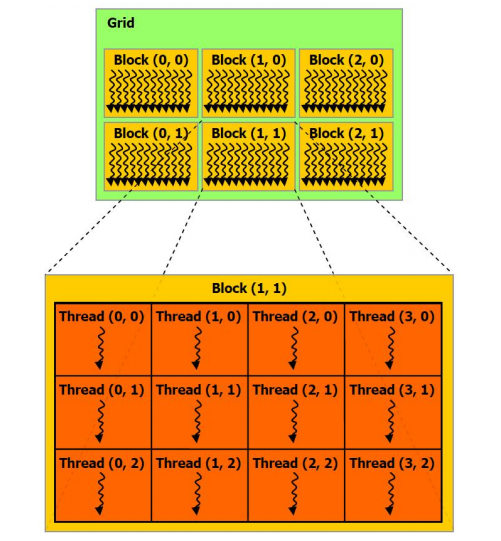
\includegraphics[scale=0.55]{images/cuda1.png}
	\caption{Organisierung von Threads in Blocks in Grids REF}
	\label{img:cuda1}
\end{figure}

\begin{itemize}
	\item TODO: Beispiel anhand von Vektor / Matrix, warps?
\end{itemize}

Zur Speicherverwaltung nutzt cuda sowohl \textit{global memory} als auch \textit{shared memory}. Sofern nicht expliziert \textit{shared memory} verwendet wird, werden alle Daten im \textit{global memory} gehalten. Gerade bei vielen parallelen Lese- / Schreibzugriffen kann hier eine hohe Latenz auftreten, wenn viele Threads auf die gleichen Adressen zugreifen. Aus diesem Grund empfiehlt es sich, die benötigten Daten von dem \textit{global} in den \textit{shared memory} zu kopieren. Der \textit{shared memory} wird von allen Threads in einem Block geteilt. Beim Kopieren der Daten muss also wieder ein Index berechnet werden, um die korrekten Daten dem jeweiligen Block zuzuordnen. Weiterhin ist zu beachten, dass nicht beliebig viel \textit{shared memory} allokiert werden kann: Je nach Grafikkarten stehen pro Block zwischen 16 und 48 KiB Speicher zur Verfügung.

\subsection{Beispiel?}